\documentclass[11pt,a4paper]{article}
\usepackage[utf8]{inputenc}
\usepackage[spanish]{babel}
\usepackage{amsmath}
\usepackage{amsfonts}
\usepackage{amssymb}
\usepackage{graphicx}
\usepackage[left=2cm,right=2cm,top=2cm,bottom=2cm]{geometry}
\usepackage{listings}
\usepackage[hidelinks]{hyperref}
\usepackage{lscape}
\usepackage{rotating}
\usepackage{pdflscape}

\lstset{
basicstyle=\ttfamily,
frame=single,
language=SQL,
tabsize=2,
showstringspaces=false,
literate=%
    {á}{{\'a}}1
    {é}{{\'e}}1
    {è}{{\`e}}1
    {í}{{\'i}}1
    {ó}{{\'o}}1
    {ú}{{\'u}}1
}

\begin{document}

\begin{titlepage}
	\title{{\Huge \textbf{Práctica 4 - Bases de Datos 2}}}
	\author{
	  Hayk Kocharyan\\
	  757715@unizar.es
	  \and
	  Juan José Tambo Tambo\\
	  755742@unizar.es
	  \and
	  Pedro Tamargo Allué\\
	  758267@unizar.es
	  \and
	  Jesús Villacampa Sagaste\\
	  755739@unizar.es
	}
	\date{\today}
	
	\clearpage\maketitle
	\thispagestyle{empty}
	\tableofcontents
	\listoffigures
\end{titlepage}

\section{Esfuerzos invertidos}

\begin{itemize}
\item Hayk:
\item Juan José:
\item Pedro:
\item Jesús:
\end{itemize}

\section{Modelo conceptual}

\textbf{Aquí explicaremos el diagrama er de banquito, para que lo tengan presente (Figura \ref{fig:diagramaer}).}

\section{Entorno de trabajo y ejecución}

\textbf{Aquí le explicaremos que usamos visual code con maven y le explicaremos como se ejecuta.}

\section{Generación de esquema lógico con JPA}

\textbf{Aquí explicaremos como hemos desarrollado el esquema lógico desde 0 con JPA.}

\section{Adopción de un esquema lógico preexistente con JPA}

\textbf{Aquí le explicaremos el proceso de acomodación del esquema relacional de la base de datos con JPA. Le explicaremos lo del \emph{validate} y le mostraremos nuestros problemas.}

\section{Consultas con JPA}

\textbf{Aquí se expondrán las consultas, con su código SQL, JPQL, Criteria API}.

\section{Apéndice 1: Figuras}

\begin{landscape}
\begin{figure}
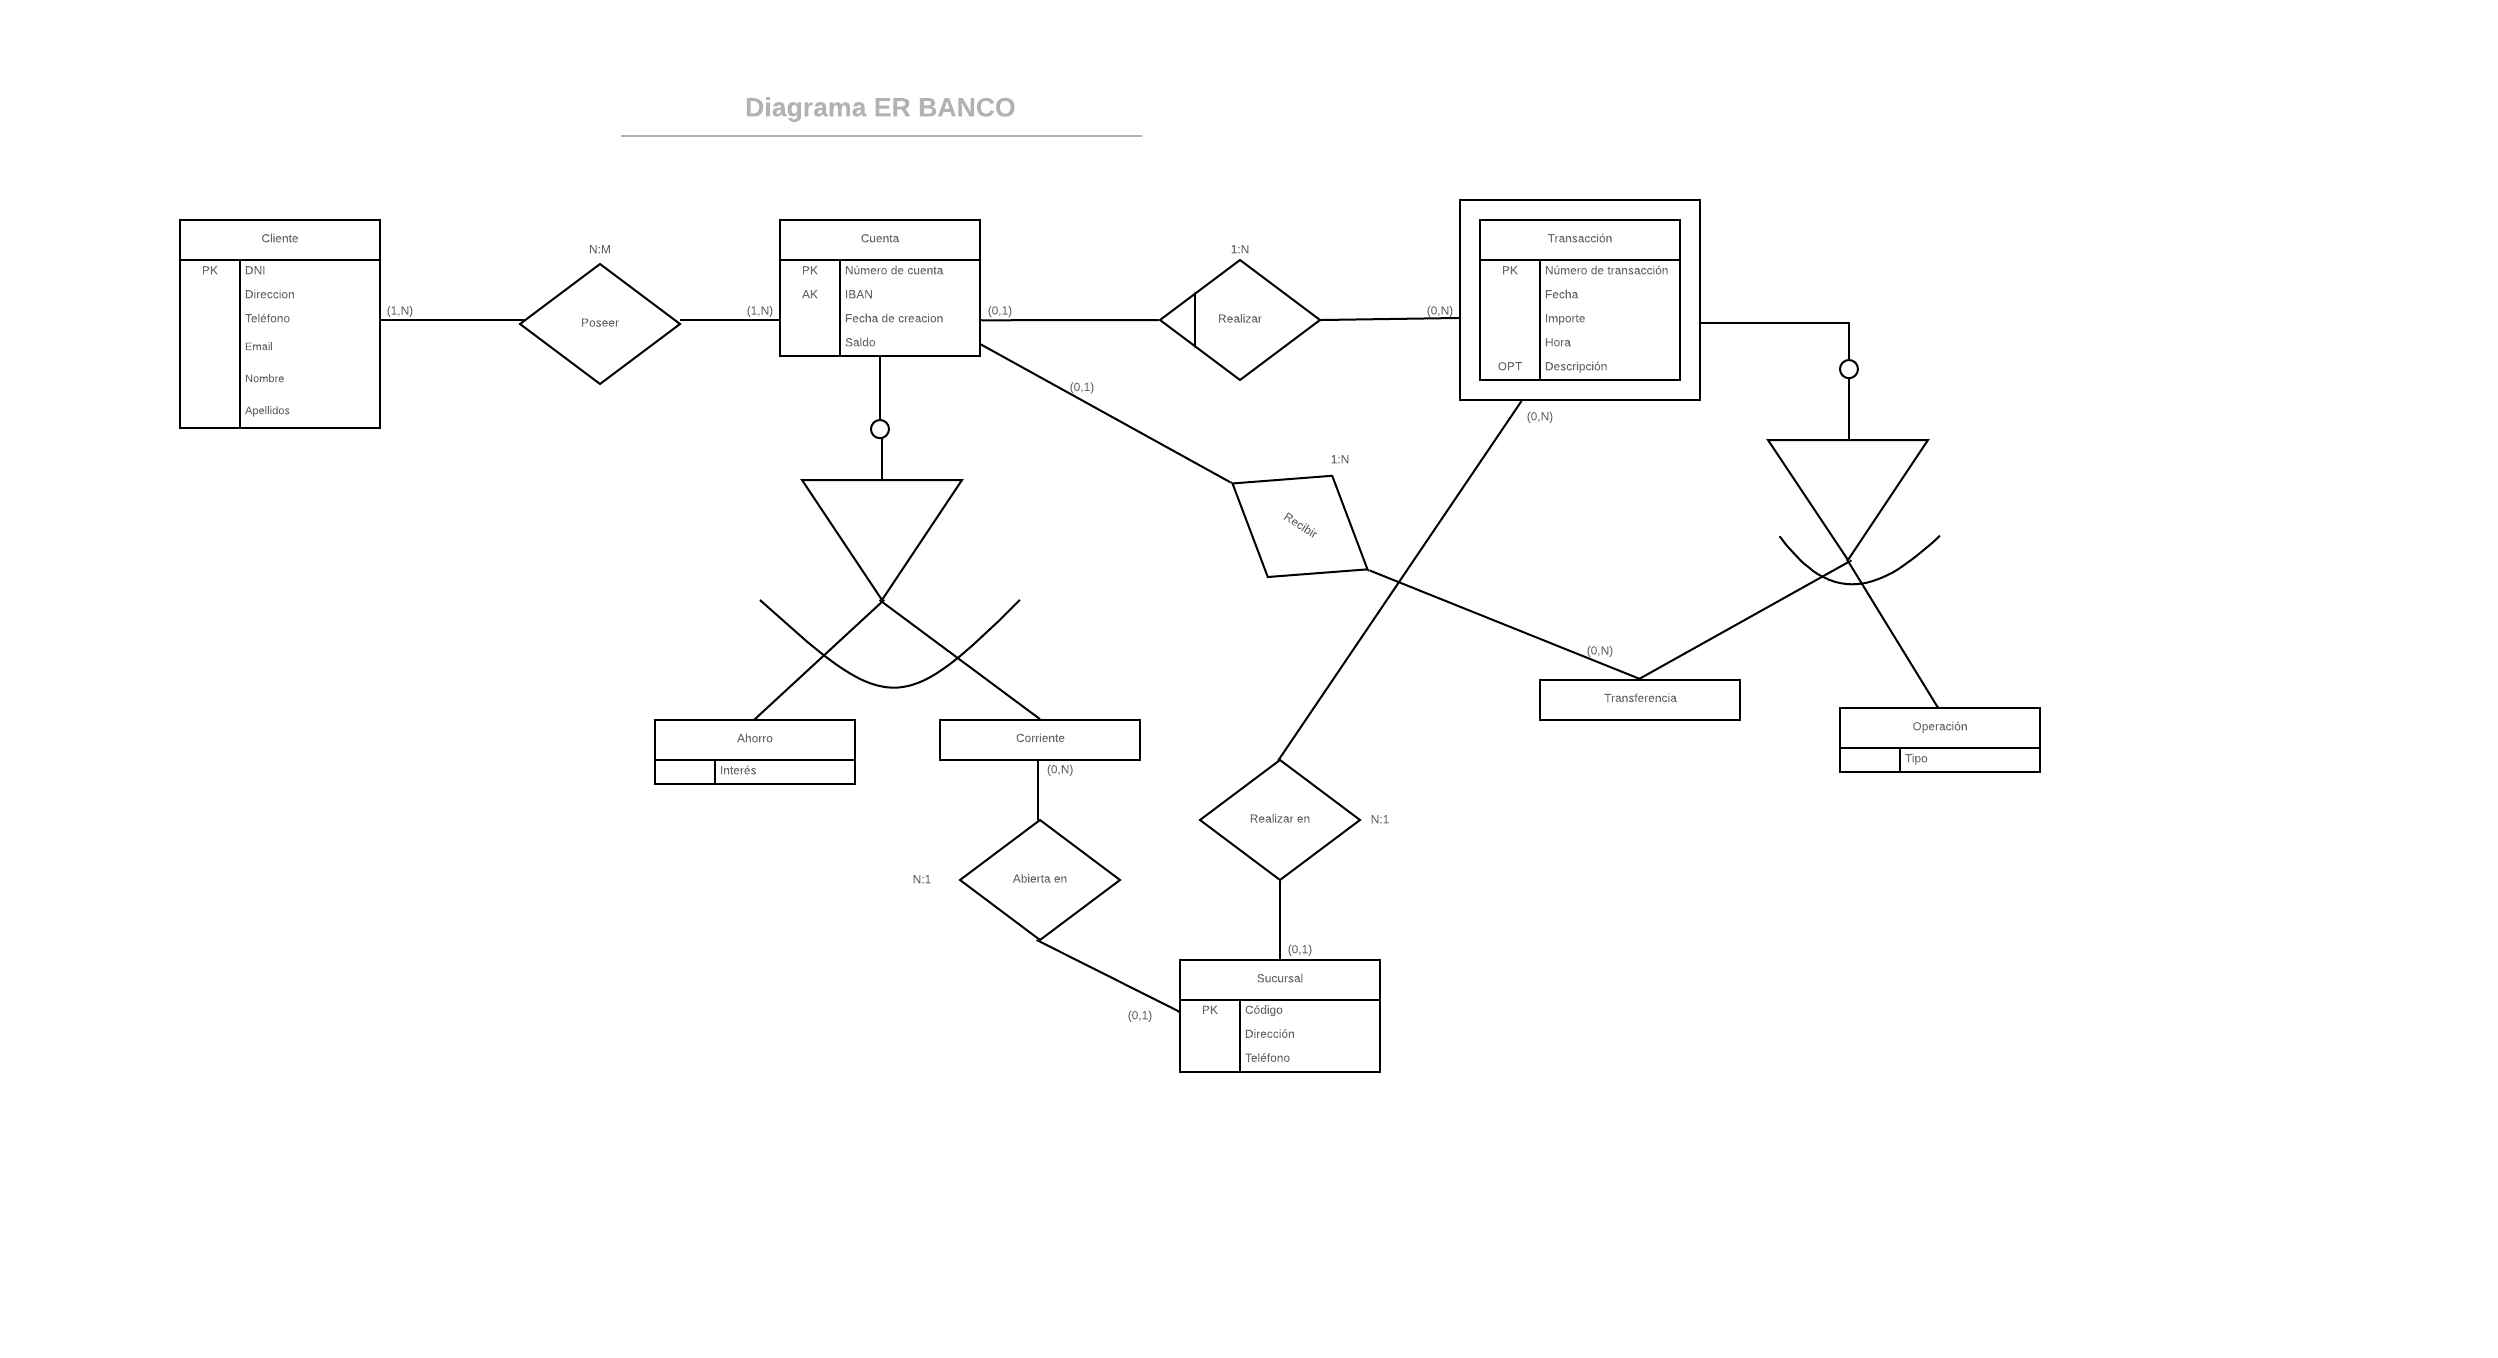
\includegraphics[scale=0.75]{images/diagramaer.png}
\caption{Diagrama ER de la Base de Datos bancaria de \emph{Banquito}}
\label{fig:diagramaer}
\end{figure}
\end{landscape}

\end{document}